\documentclass[final, hyperref={pdfpagelabels=false}]{beamer}

\usepackage{amsmath,amssymb,amsfonts,amsthm,tipa,multirow,rotating,latexsym,graphicx,psfrag,hyperref}

\usepackage[latin1]{inputenc}
\usefonttheme[onlymath]{serif}
\boldmath
\usepackage[orientation=portrait,size=a0,scale=1.5,debug]{beamerposter}
\newcommand{\jl}{$\frac{}{}$}

\mode<presentation>{
	\usetheme{I6dv}
	}


\title{Real Time Tracking and Analysis of Election Polling in Israel}
\author[Sidi]{Jonathan Sidi}
\institute[Hebrew University, Statistics Department]{ISA Conference 2015}
\date{May 26th, 2015}
\begin{document}
\begin{frame}{}
	\begin{columns}[t]
		\begin{column}{.3\linewidth}
			\begin{block}{Motivation}
				\begin{itemize}
					\item News outlets report to the public increasingly larger amounts of information throughout each successive election cycle. 
					\item One of the most important items is polls they publish which help inform the public and play an important role of shaping an opinion on which party to vote for on Election Day. 
					\item Tracking the daily stream of polling results from media outlets and cross checking the pollsters which conduct the polls and their sampling error is a labor intensive task that is not on the minds of the general public. 
					\item Creating an online interactive framework that centralizes the polling information in real time for the simple voter has turned into a necessity.
										
				\end{itemize}
			\end{block}
		\end{column}
		\begin{column}{.3\linewidth}			
			\begin{block}{Interactive Polling Analysis Layout} 
				 \begin{itemize}
					 \item An open source web application is presented which gathers continuously updated polling information to one location. 
					 \item The user is given all the available information to ascertain the current state of the public opinion, as represented in the polls, through an interactive polling analysis layout.
				 	\item Different types of plots can be created through filtering elections, parties, party attributes, publishers, pollster and dates which include published polling results starting from 2003.
				 	\item  A mandate simulator which constructs confidence limits of mandates for each party as reported by the pollsters.
				 	\item A coalition white board to create party coalitions and see if their parties of interest can pass 60 mandates to form a government
				 \end{itemize} 
			\end{block}
		\end{column}
		\begin{column}{.3\linewidth}
			\begin{block}{Data}
			\begin{itemize}
			\item Daily historical published election polling results from the 2003, 2006, 2009,2013 elections and daily polling publication from the 2015 election are stored and managed by Project 61 on the Google spreadsheets platform.
			\item The application automatically imports the data and organizes it using R and the web application is generated using Shiny by RStudio 
			\item Data can be filtered by the following variables
			\begin{itemize}
			\item Time: Election Year, Days Left to Election, Date
			\item Party: Party, Block Affiliation, Genealogy
			\item Results: Mandates, Results, Error
			\item Poll: Publisher, Pollster
			\end{itemize}
			\item Graphs displayed in both Hebrew and English
			\item All graphs can be downloaded and shared
			\end{itemize}
			 
			\end{block}
		\end{column}
	\end{columns}
	\begin{columns}[t]		
		\begin{column}{.45\linewidth}
			\begin{block}{Up to Date Polls}
				\begin{figure}[h]
				\centering
				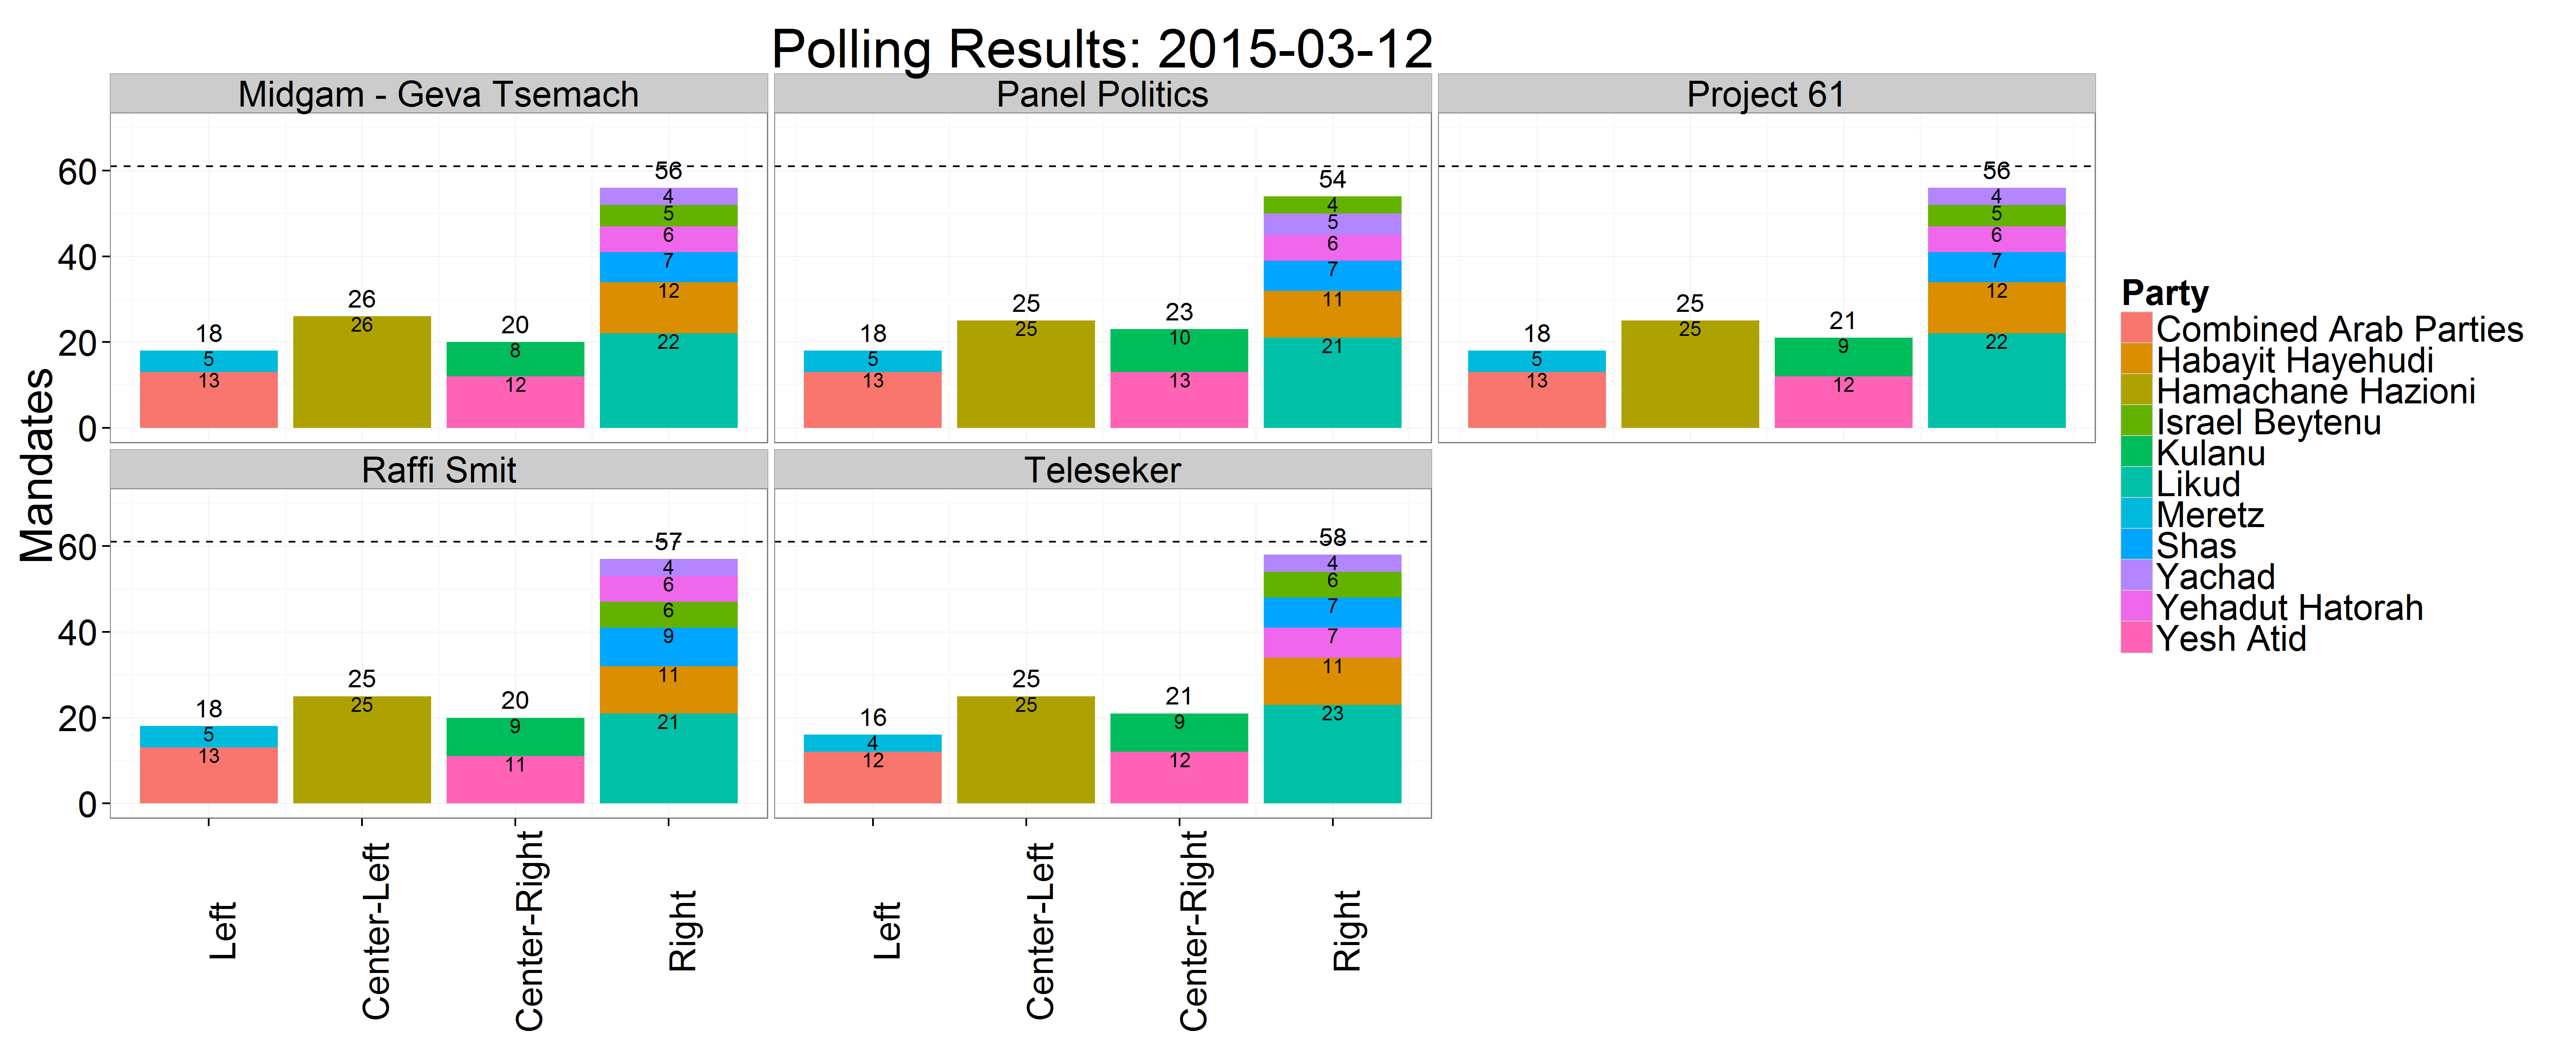
\includegraphics[width=1\linewidth]{../www/LastDayPlot}
				\caption{The latest polling day results published in the media and the prediction made using the Project 61 weighting schemes. The parties are stacked into blocks to see which block has best chance to create a coalition.}
				\label{fig:LastDayPlot}
				\end{figure}
			\end{block}

			\begin{block}{Mandate Simulator}
				\begin{figure}[h]
					\centering
					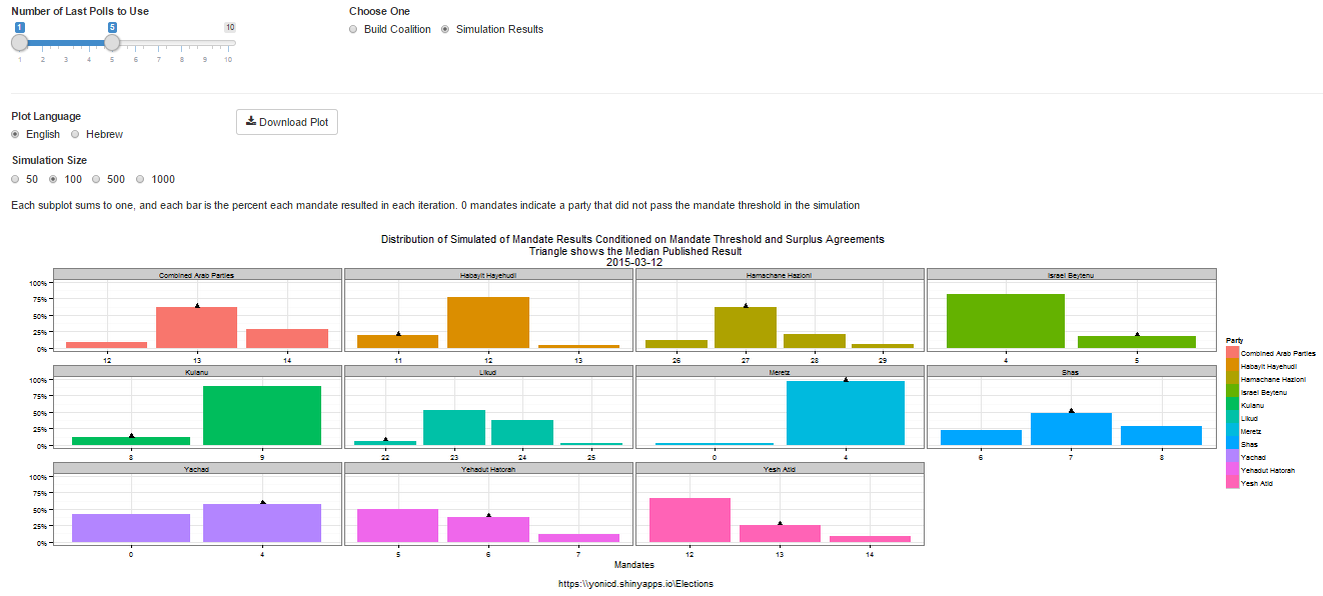
\includegraphics[width=.9\linewidth]{../www/sim_screen_grab}
					\caption{In order to frame the polling results in their natural range of uncertainty and not as a seemingly absolute point estimate, a bootstrap simulation is performed using the published sampling error to reproduce the distribution of mandates for each party. The simulation takes into account up to 10 recent polls, the mandate surplus agreements using the Hagenbach-Bischoff quota method and the mandate threshold limit (4), giving the final statistic and its standard error. The distributions are plotted per party and compared to the location of the median published results in the media.}
					\label{fig:sim_screen_grab}
				\end{figure}				
			\end{block}
			
			\begin{block}{Coalition White board}
				\begin{figure}[h]
					\centering
					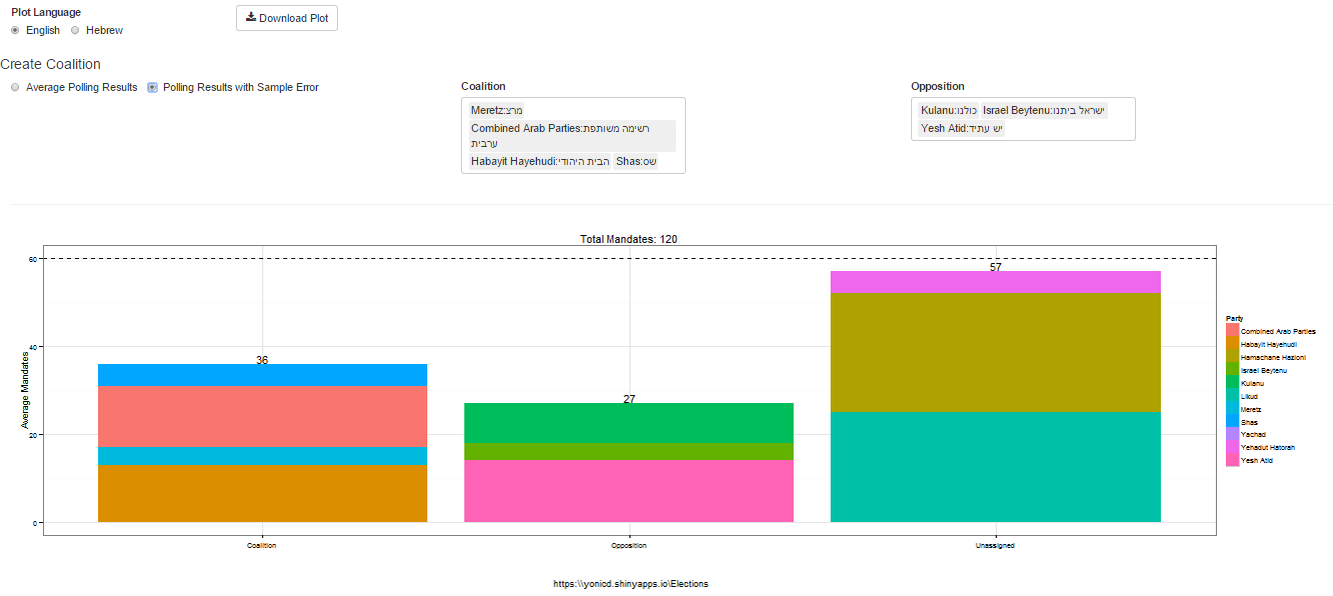
\includegraphics[width=.8\linewidth]{../www/coal_screen_grab}
					\caption{Create coalitions based on either the simulated distribution or actual published polls and see who can pass 60 mandates.}
					\label{fig:coal_screen_grab}
				\end{figure}				
			\end{block}
		\end{column}
		
		\begin{column}{.45\linewidth}
			\begin{block}{Interactive Graphs}
			An interactive polling analysis layout where the user can filter elections, parties, publishers and pollster, dates and create different types of plots using any variable as the x and y axis. The user can choose to include in the plots Elections, 2003 to 2015, and the subsequent filters are populated with the relevant parties, pollsters and publishers relevant to the chosen elections.
				\begin{figure}[h]
					\centering
					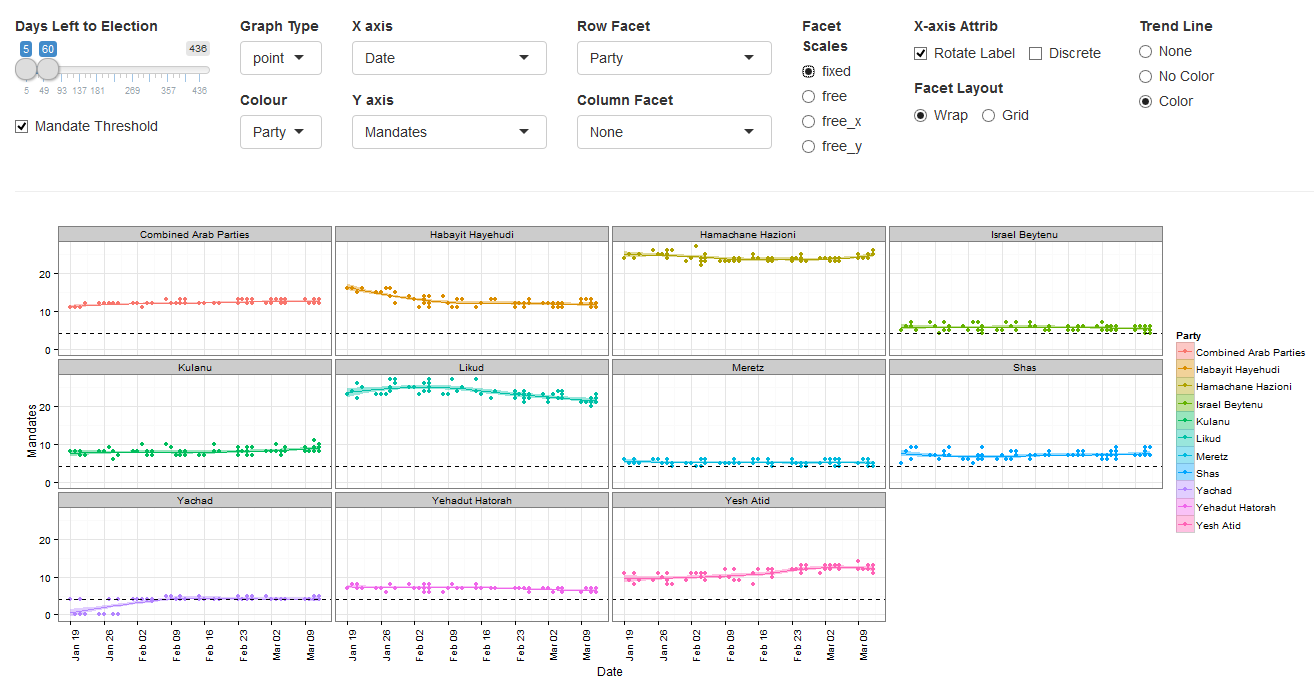
\includegraphics[width=.85\linewidth]{../www/pad_screen_grab}
					\caption{60 day trend (estimated with loess smoother) of mandates published by each pollster by party}
					\label{fig:pad_screen_grab}
				\end{figure}

				\begin{figure}[h]
					\centering
					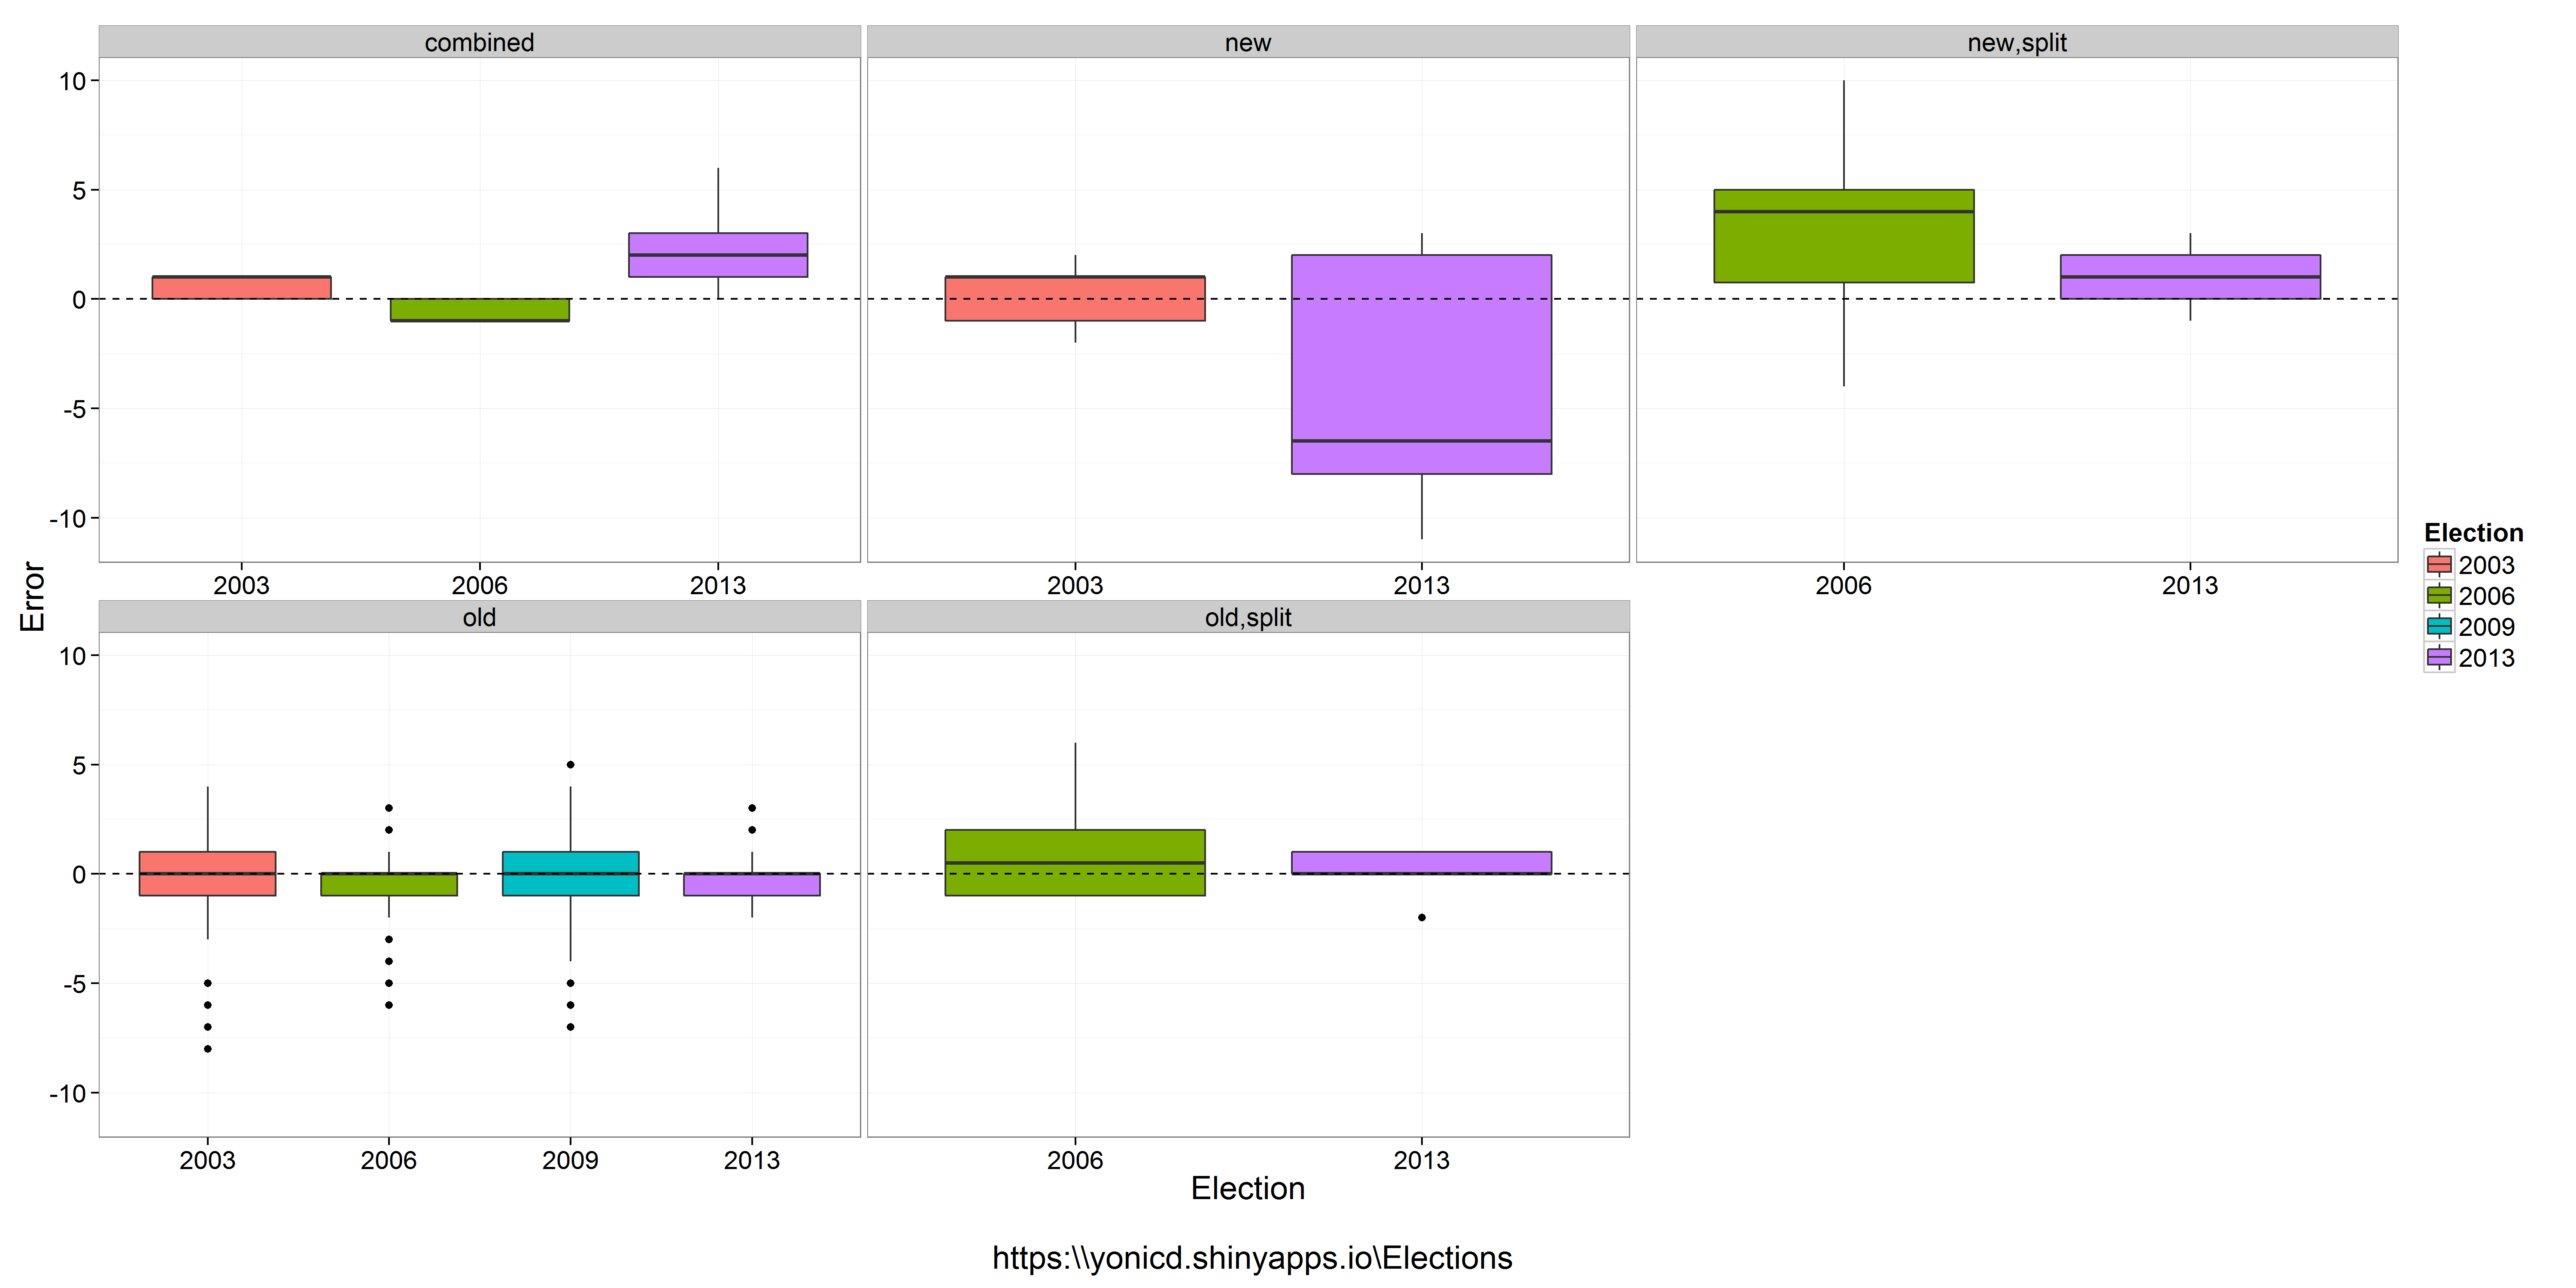
\includegraphics[width=.75\linewidth]{../www/ElectionPlot_longitudinal}
					\caption{Comparing distribution of pollster errors across elections, 10 days prior end of polling, by splitting the parties into five groups compared to previous election: old party,new party, combined (combination of two or more old parties), new.split (new party created from a split of a party from last election), old.split (old party that was a left from the split).}
					\label{fig:ElectionPlot_longitudinal}
				\end{figure}	
%				\begin{figure}[h]
%					\centering
%					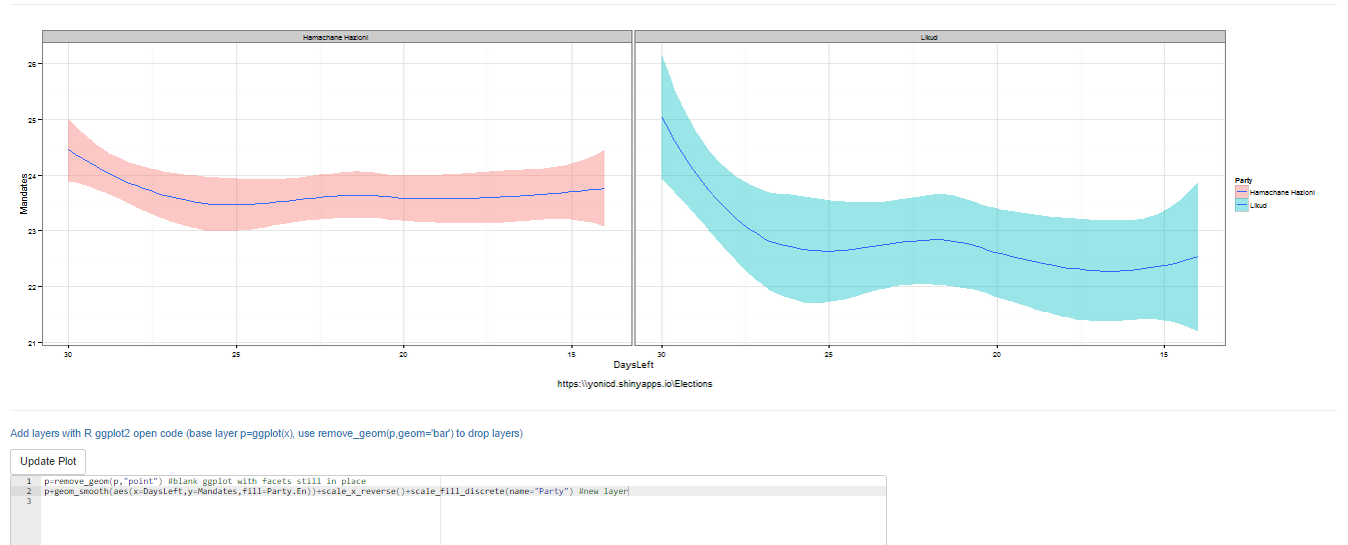
\includegraphics[width=.75\linewidth]{../www/pad_screen_grab_ace_remove_geom}
%					\caption{Advanced plots can be generated with free hand code in an editor console. The user can add layers to the base plot, or remove any of the original layers and make a plot from scratch.}
%					\label{fig:pad_screen_grab_ace_remove_geom}
%				\end{figure}			
				\begin{figure}[h]
					\centering
					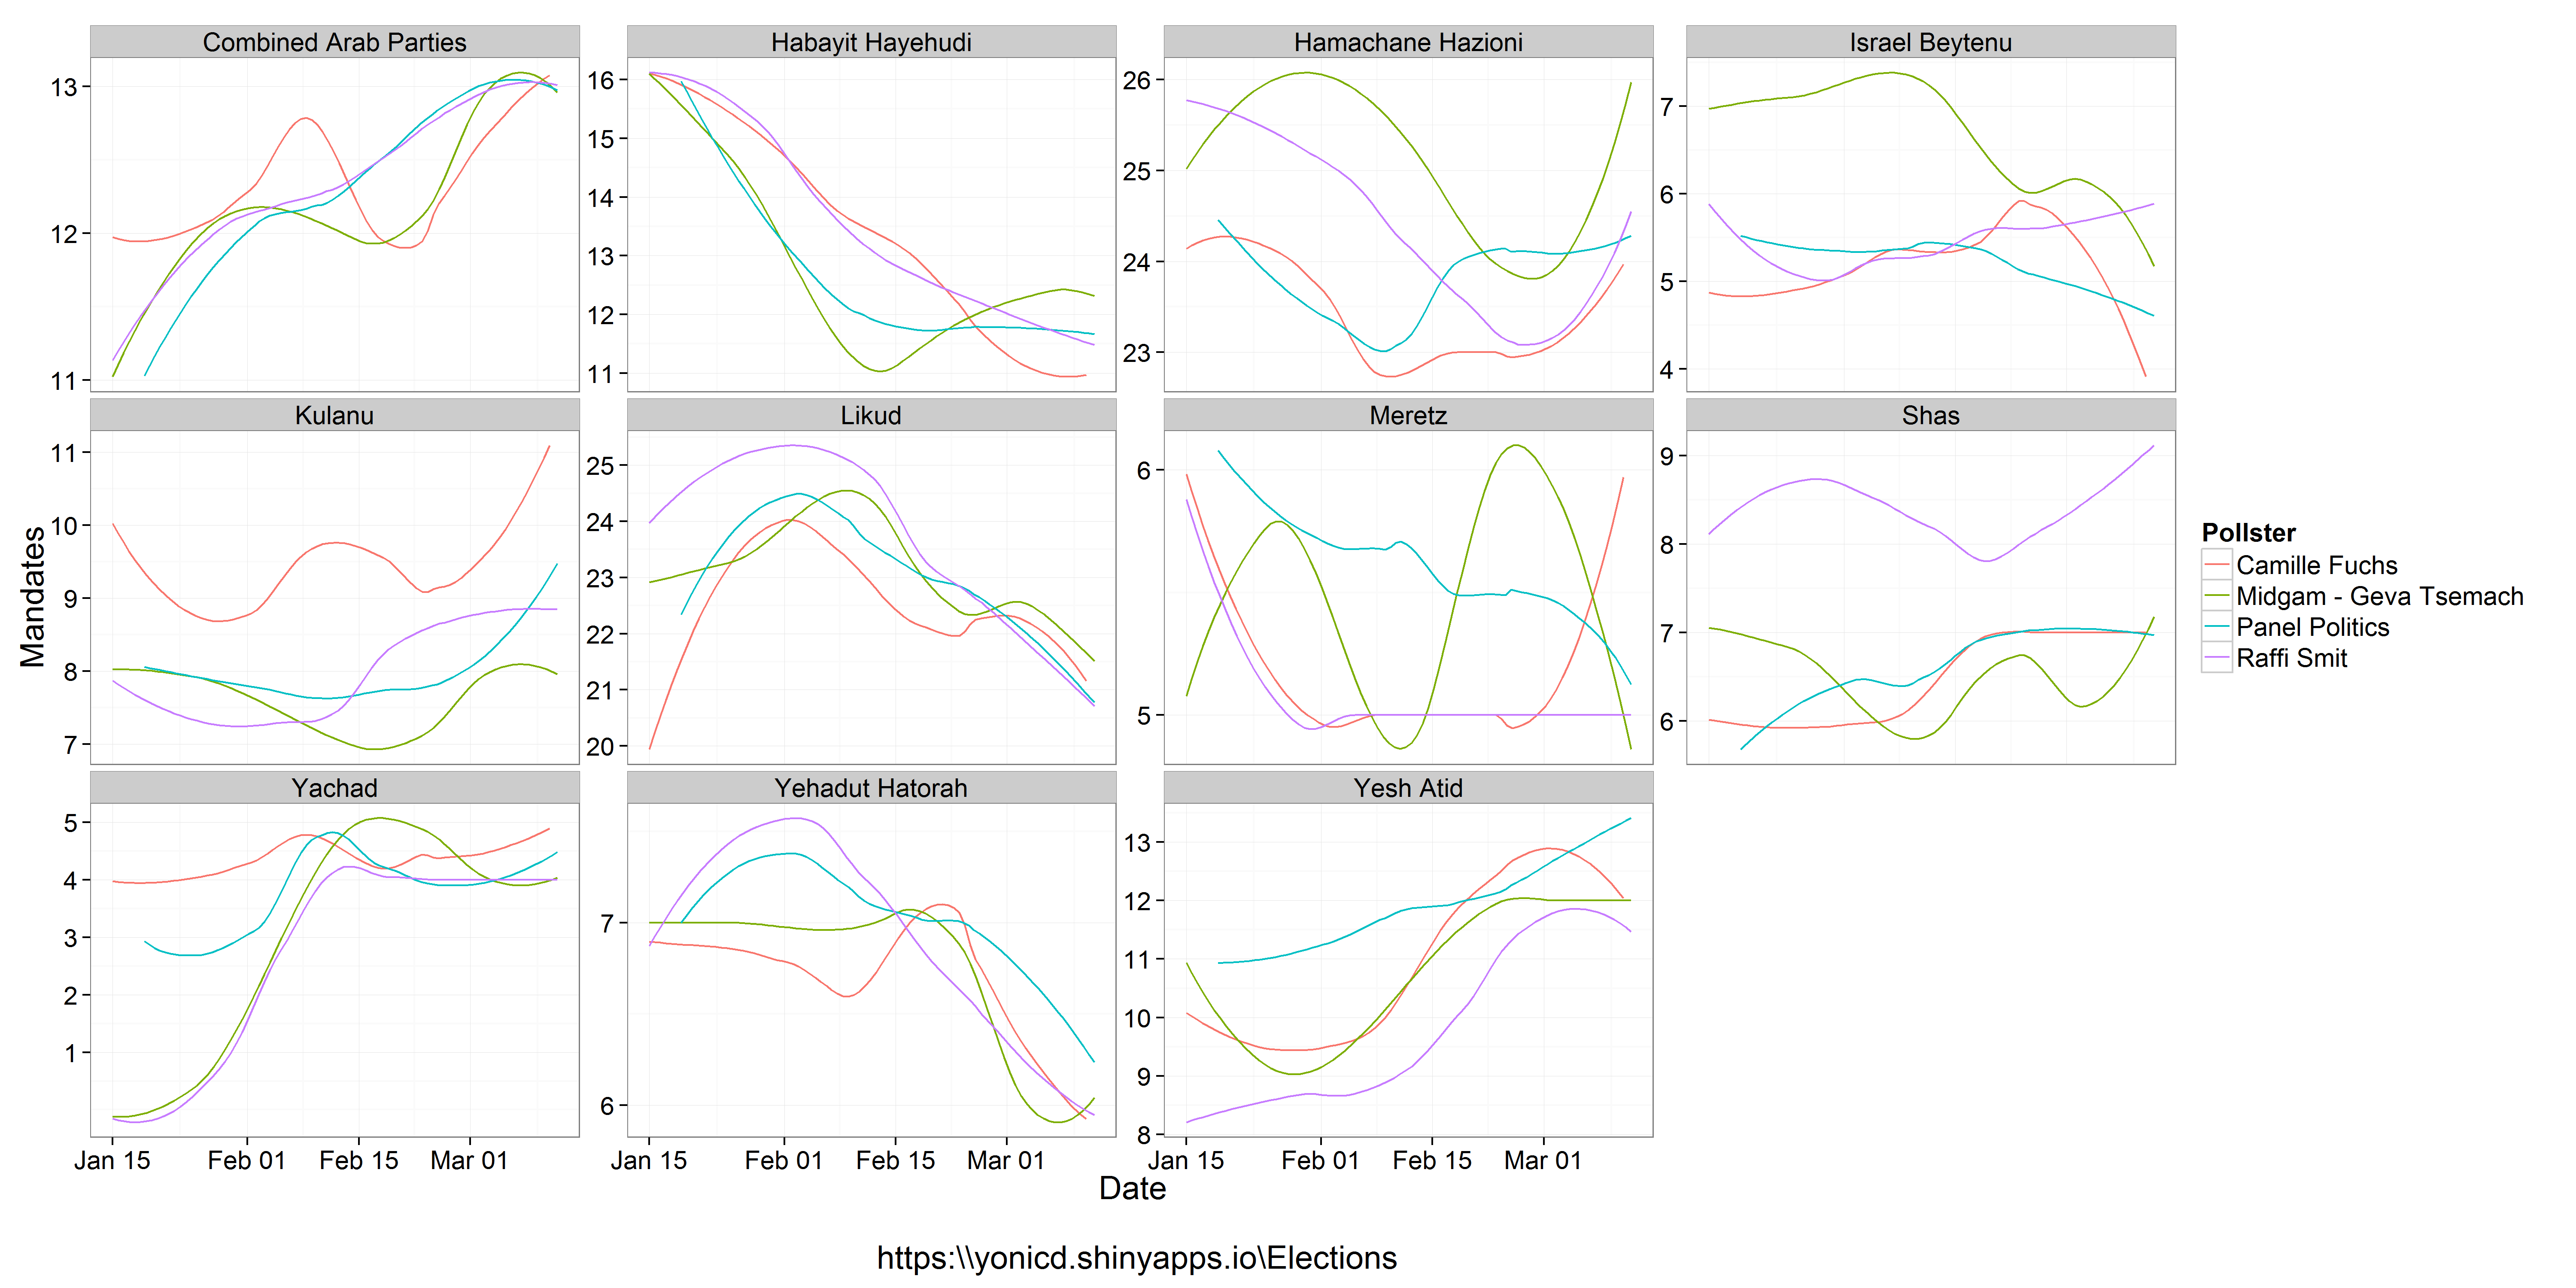
\includegraphics[width=.75\linewidth]{../www/ElectionPlot_trend}
					\caption{Comparison of pollster results within parties, to locate variability in public opinion, or pollster estimation bias towards a specific party.}
					\label{fig:ElectionPlot_trend}
				\end{figure}	
			\end{block}
		\end{column}
		
	\end{columns}
\end{frame}
\end{document}